\documentclass{article}[10pt]
\usepackage[pdftex]{graphicx}
\usepackage{amsfonts}
\usepackage[italian]{babel}
\usepackage{graphicx}

%****************enlarge layout
\textheight     243.5mm
\topmargin      -20.0mm
\textwidth      480pt
\hoffset        -80pt
%*****************theorems and such
\newcounter{esnu}
\newenvironment{esercizio}{\medskip \noindent {\bf Esercizio\addtocounter{esnu}{1} \arabic{esnu}}}{}
\pagestyle{empty}
\newcommand{\liff}{\mathrel{\leftrightarrow}}   % Logical IFF Symbol
\newcommand{\metaiff}{\Longleftrightarrow}      %iff in metatheory

\begin{document}

%\begin{tabular}{llclcr}
% \hspace{-35pt} &{\bf COGNOME:} & \hspace{100pt}        &{\bf NOME:}    & \hspace{100pt}        &{\bf MATRICOLA:}%\hspace{35pt} \\
%\hline
%\end{tabular}
\begin{center} {\bf Esame di Programmazione II, 26 giugno 2017}\end{center}
%\`

Si consideri la seguente gerarchia di classi, che implementa le pizze
di un'ipotetica pizzeria:

\begin{center}
  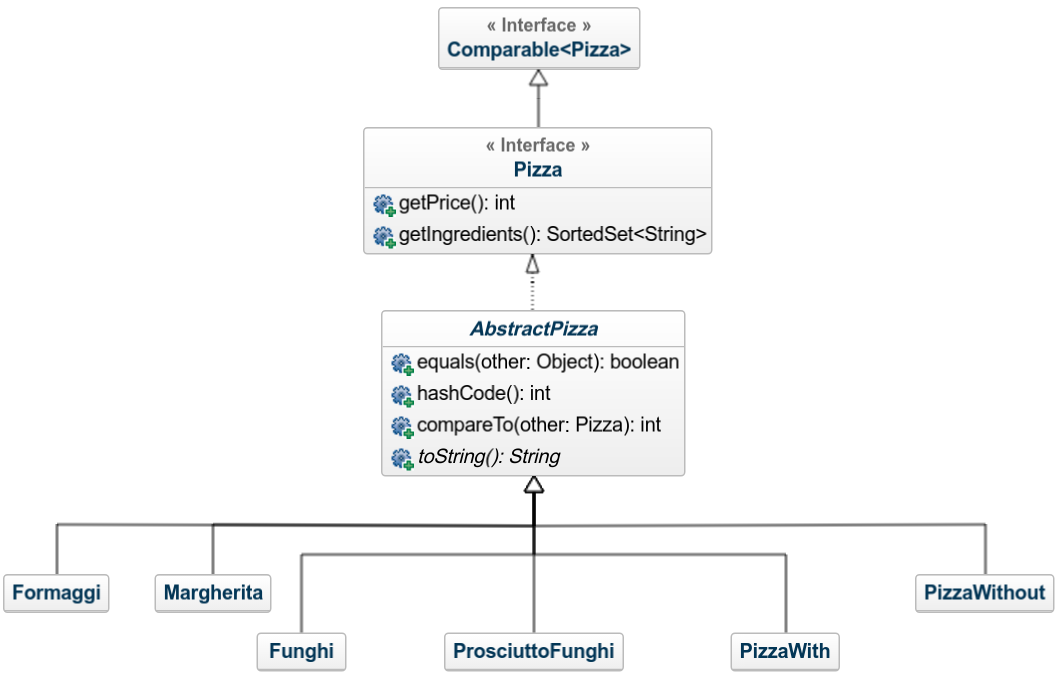
\includegraphics[scale=.35,clip=false]{hierarchy.png}
\end{center}

\noindent
Si noti che \texttt{Pizza} \`e un'interfaccia che estende
l'interfaccia \texttt{Comparable<Pizza>} della libreria Java standard.
Inoltre la classe \texttt{AbstractPizza} \`e astratta: implementa
in modo \texttt{final} i metodi
\texttt{equals}, \texttt{hashCode} e \texttt{compareTo} e dichiara
\texttt{toString} astratto. Due pizze sonno considerate uguali se e solo se
hanno gli stessi ingredienti. Sono messe in ordine (\texttt{compareTo}) rispetto
all'ordine alfabetico della concatenazione dei rispettivi ingredienti.

\begin{esercizio}
\textbf{[8 punti]}
Si implementino l'interfaccia \texttt{Pizza} e la classe astratta
\texttt{AbstractPizza}.
I metodi \texttt{equals}, \texttt{hashCode} e \texttt{compareTo}
devo essere consistenti fra di loro. Si eviti di implementare
\texttt{hashCode} in modo costante, perch\'e sarebbe inefficiente.
\end{esercizio}

\begin{esercizio}
\textbf{[3 punti]}
Si completi la seguente implementazione della pizza \texttt{Margherita}:

{\small\begin{verbatim}
public final class Margherita extends AbstractPizza {
  final static Margherita INSTANCE = new Margherita(); // unico oggetto esistente
  private Margherita() {}

  .. stampandola si ottiene "Margherita", i suoi ingredienti sono "tomato" e "mozzarella", il costo 5 euro
}
\end{verbatim}}

\noindent
Si faccia lo stesso anche per le classi \texttt{Formaggi} (costa 8 euro
e ha come ingredienti ``mozzarella'', ``parmesan'' e ``gorgonzola''),
\texttt{Funghi} (7 euro, ``tomato'',
``mozzarella'' e ``mushrooms'') e \texttt{ProsciuttoFunghi}
(8 euro, ``tomato'', ``mozzarella'',
``mushrooms'' e ``ham''). A questo punto il men\`u della pizzeria \`e pronto:
%
{\small\begin{verbatim}
public class Menu {
  public final static Pizza MARGHERITA = Margherita.INSTANCE;
  public final static Pizza FUNGHI = Funghi.INSTANCE;
  public final static Pizza FORMAGGI = Formaggi.INSTANCE;
  public final static Pizza PROSCIUTTO_FUNGHI = ProsciuttoFunghi.INSTANCE;
}
\end{verbatim}}
%
\end{esercizio}

\begin{esercizio}
\textbf{[10 punti]}
La classe \texttt{PizzaWith} rappresenta la modifica di un'altra pizza,
con l'aggiunta di un singolo ingrediente. Tale ingrediente
non deve gi\`a essere fra quelli della pizza a cui lo si sta aggiungendo,
perch\'e in tal caso non avrebbe senso aggiungerlo.
Aggiungendo l'ingrediente, il prezzo della pizza aumenta e la sua stampa
\`e espansa con l'ingrediente aggiunto. Si completi l'implementazione seguente:

{\small\begin{verbatim}
public class PizzaWith extends AbstractPizza {
  ...
  // costruisce la pizza ottenuta da base aggiungendo l'ingrediente indicato, che costa
  // il prezzo extra indicato. Se l'ingrediente era gia' fra quelli della pizza base,
  // deve lanciare un'eccezione di classe IllegalPizzaModificationException
  public PizzaWith(Pizza base, String addedIngredient, int extraPrice) { ... }

  @Override public String toString() {
    ... ritorna il toString() di base concatenato con "with" e l'ingrediente aggiunto
  }

  @Override public SortedSet<String> getIngredients() { ... ha gli ingredienti di base piu' quello aggiunto }
  @Override public int getPrice() { ... ha il prezzo di base piu' il prezzo extra da aggiungere }
}
\end{verbatim}}

\noindent
Si faccia la stessa cosa per la classe \texttt{PizzaWithout}, che rappresenta
una pizza ottenuta eliminando un ingrediente da un'altra pizza.
Questa volta si ottiene una \texttt{IllegalPizzaModificationException} se la pizza di partenza non conteneva
l'ingrediente che si vuole togliere.
\end{esercizio}

\begin{esercizio}
\textbf{[2 punti]}
Si implementi l'eccezione \texttt{IllegalPizzaModificationException}.  
\end{esercizio}

\begin{esercizio}
\textbf{[5 punti]}
Si implementi un ordine della pizzeria, che contiene la sequenza
delle pizze che si ordina:
%
{\small\begin{verbatim}
public class Order {
  ...
  public Order(Pizza... pizzas) { ...prende nota delle pizzas ordinate }

  @Override public String toString() {
    ... ritorna la stampa delle pizze ordinate con i prezzi di ciascuna
    e in fondo il prezzo totale dell'ordine (si veda esempio in basso)
  }

  public int getPrice() { ... ritorna il prezzo totale dell'ordine }
}
\end{verbatim}}
  
\end{esercizio}

\vspace*{2ex}
\hrule

\mbox{}\\

Se tutto \`e corretto, l'esecuzione del programma:
{\scriptsize\begin{verbatim}
public class Main {
  public static void main(String[] args) {
    Pizza p1 = Menu.FUNGHI; Pizza p2 = Menu.MARGHERITA; Pizza p3 = Menu.PROSCIUTTO_FUNGHI;
    Pizza p4 = new PizzaWithout(p1, "mushrooms", 2); // p4 e' p1 con la rimozione dei funghi
    Pizza p5 = new PizzaWith(p4, "mushrooms", 2); // p5 e' p4 con l'aggiunta dei funghi

    Set<Pizza> allFiveSet = new HashSet<>();
    allFiveSet.add(p1); allFiveSet.add(p2); allFiveSet.add(p3); allFiveSet.add(p4); allFiveSet.add(p5);

    List<Pizza> allFiveList = new LinkedList<>();
    allFiveList.add(p1); allFiveList.add(p2); allFiveList.add(p3); allFiveList.add(p4); allFiveList.add(p5);

    Pizza[] allFiveArray = new Pizza[] { p1, p2, p3, p4, p5 };

    System.out.println("allFiveSet.size() = " + allFiveSet.size());
    System.out.println("allFiveList.size() = " + allFiveList.size());
    System.out.println("allFiveArray.length = " + allFiveArray.length);

    Order order = new Order(allFiveArray);
    System.out.println(order);
  }
}
\end{verbatim}}

\noindent dovr\`a stampare:

{\scriptsize\begin{verbatim}
allFiveSet.size() = COSA STAMPA?
allFiveList.size() = COSA STAMPA?
allFiveArray.length = COSA STAMPA?
----------------------
Funghi (7 euros)
Margherita (5 euros)
Prosciutto & Funghi (8 euros)
Funghi without mushrooms (5 euros)
Funghi without mushrooms with mushrooms (7 euros)
----------------------
Total price: 32 euros
\end{verbatim}}

\begin{esercizio}
\textbf{[3 punti]}
Quali numeri vengono stampati dove sopra \`e indicato \texttt{COSA STAMPA?}
\end{esercizio}

\begin{center}
\textbf{\`E possibile definire campi, metodi, costruttori e classi aggiuntive, ma solo \texttt{private}.}
\end{center}

\end{document}
